\documentclass{article}
\usepackage{listings}
\usepackage{hyperref}
\usepackage{graphicx}
\usepackage{csquotes}

\author{Tobias Dorra, Hendrik Schick}
\title{Project for Deep learning in medical imaging: Segmentation - MIC \\ \begin{large} 
Task 5: Fine tuning
\end{large}}

\begin{document}
	
	\maketitle

	\section{Task}

		The task was to fine tune the Implementation.

	\section{Implementation}

		This week, we found a bug in the method, that is responsible for building the U-Net keras model from the parameters that the \textit{Experiment Planning and Preprocessing} script from nnU-Net returned. This meant, that the model was missing one \enquote{U-Net stage} all the time. This is why this week we fixed that bug, retrained the model with the fixed architecture and evaluated the newly trained model again.

		The new model architecture is now finally to big to show it on one Din-A4 page in this report. It is attached to the moodle submission as an image file, though.

		When looking at the loss values, the performance of the model seems to have improved: While the old model had a final testing loss of $0.0148$, the final test loss for the new model is $0.0080$. Figure figure~\ref{fig:lossdev} shows, how the loss changes during the training. What is interesting in there is, that there is not too much of a difference between the training- and test loss any more. So, either, the new model architecture generalizes much better, or there is a problem with seperating the training- and test- dataset.

		\begin{figure}[htbp]
			\centering
			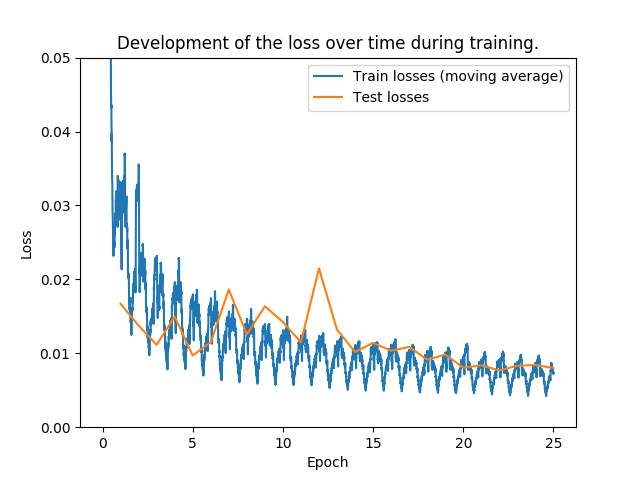
\includegraphics[width=.5\textwidth]{loss_over_time.png}
			\caption{Development of the loss during training}
			\label{fig:lossdev}
		\end{figure}

		The new average values for the intersection over union for the individual classes are the following:

		\begin{description}
			\item[Class 0] (outside): $0.99819249$
			\item[Class 1] (liver): $0.90915714$
			\item[Class 2] (cancer): $0.33424284$
		\end{description}

		So, detecting the liver now works reliably. This is also confirmed, when looking at the actual images of the predicted segmentations.

		Detecting the cancer still works not that well. It can be expected, that the IOU for the cancer is not as high as the IOU for the other two classes, because the regions with cancer are usually quite small. So if the prediction is just of by a few voxels, this already decreases the IOU score a lot. However, when looking at the individual images, for three out of the ten test images, the detected cancer does not even overlap with the real cancer at all (IOU=$0$). Those three images are also the three images in the test set, that have the smallest cancer regions. So the network might have problems detecting small tumors.

		Figure~\ref{fig:good} shows a data case where the prediction of the cancer worked well.

		Figure~\ref{fig:bad} shows a data case where the prediction worked not so well. 


		\begin{figure}[htbp]
		 	\centering
		 	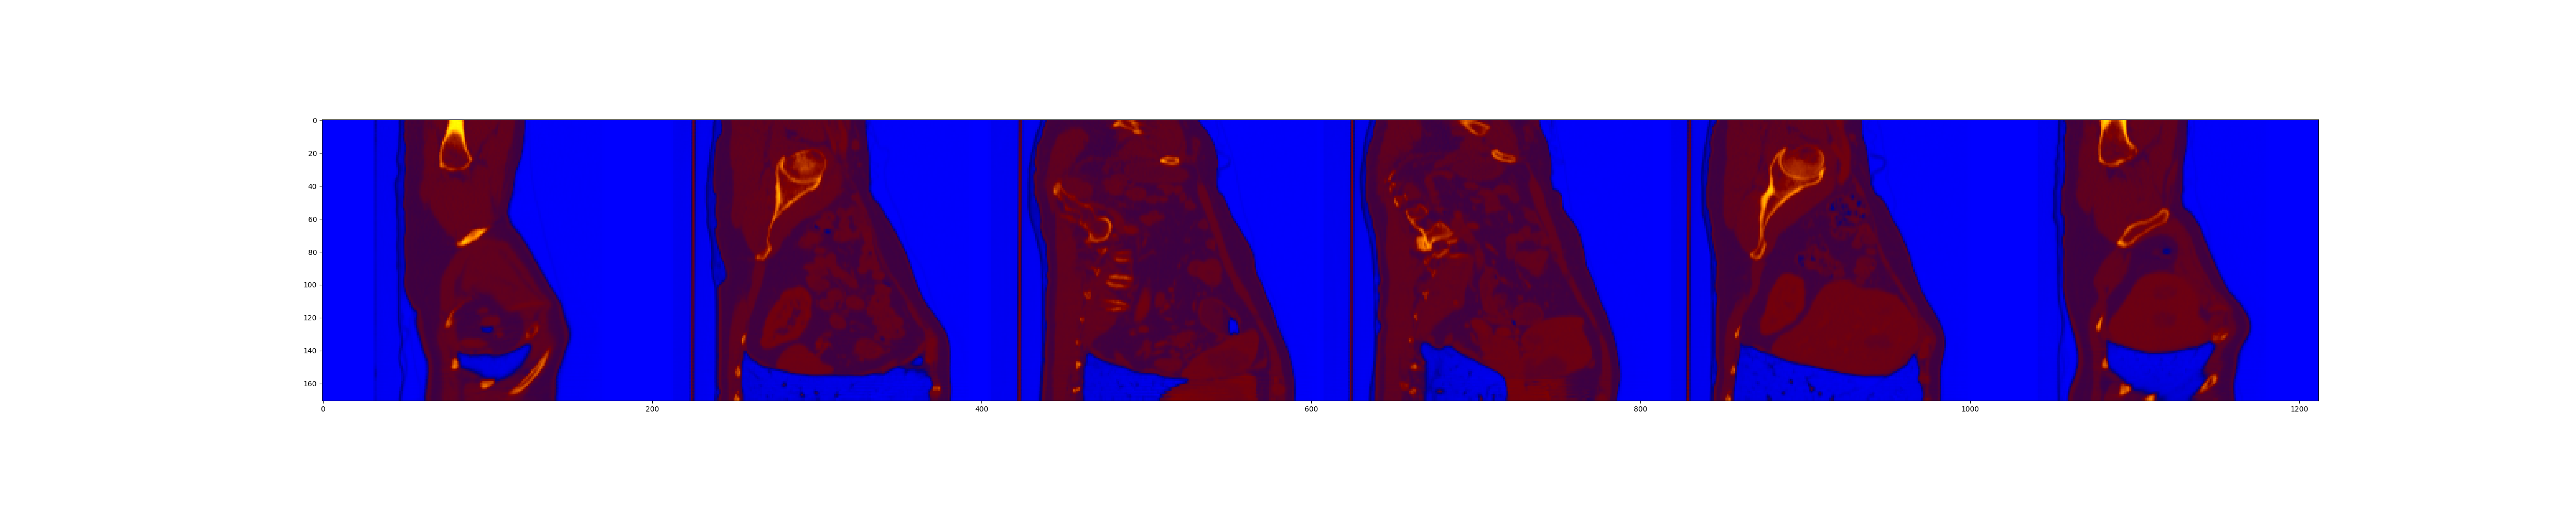
\includegraphics[width=\textwidth]{good_input.png}\\
		 	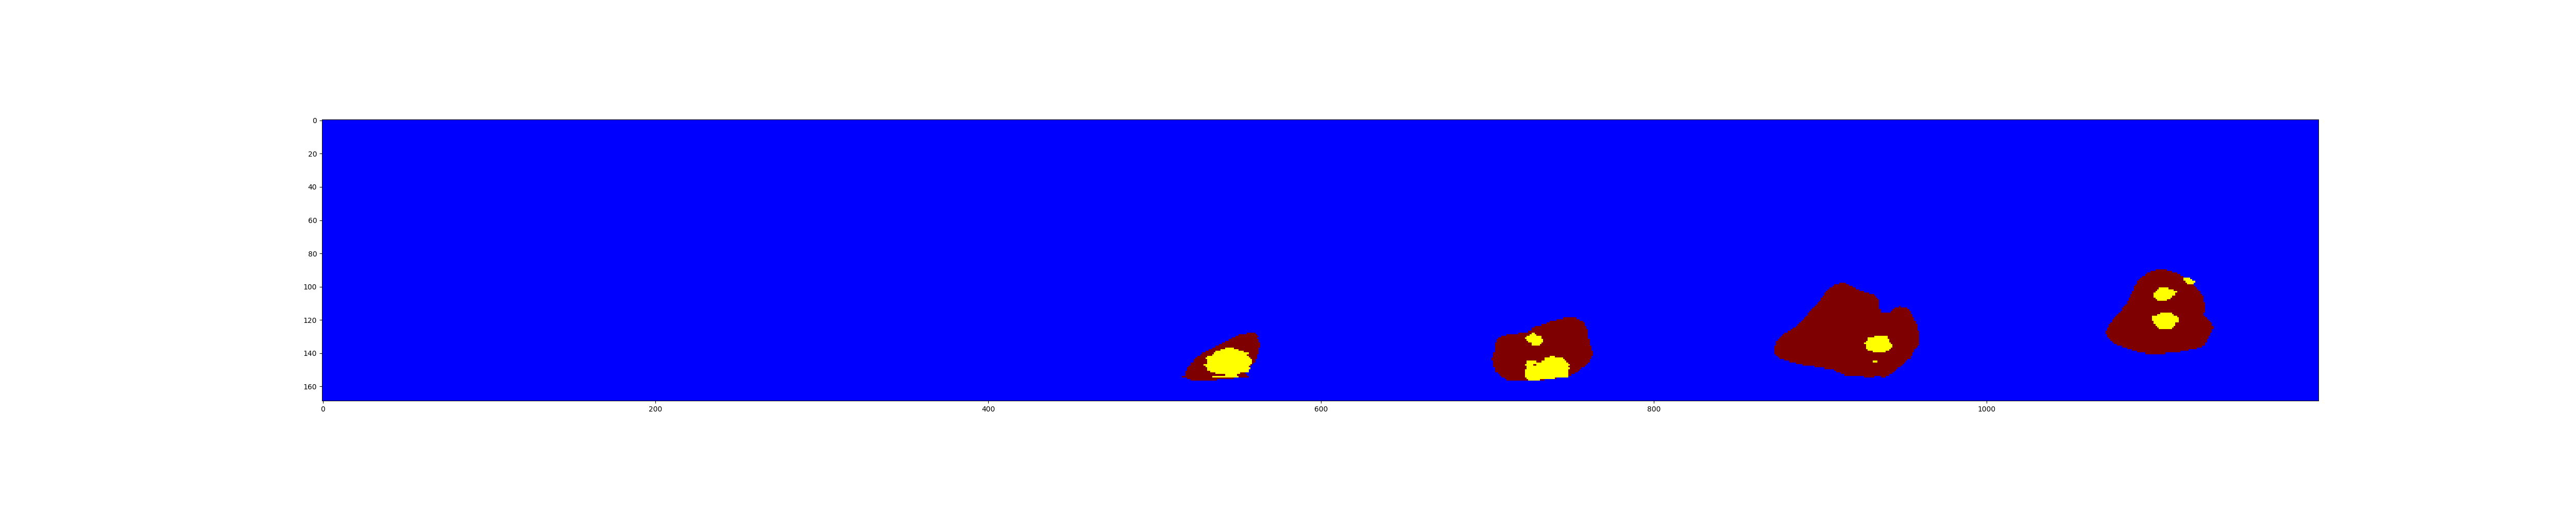
\includegraphics[width=\textwidth]{good_target.png}\\
		 	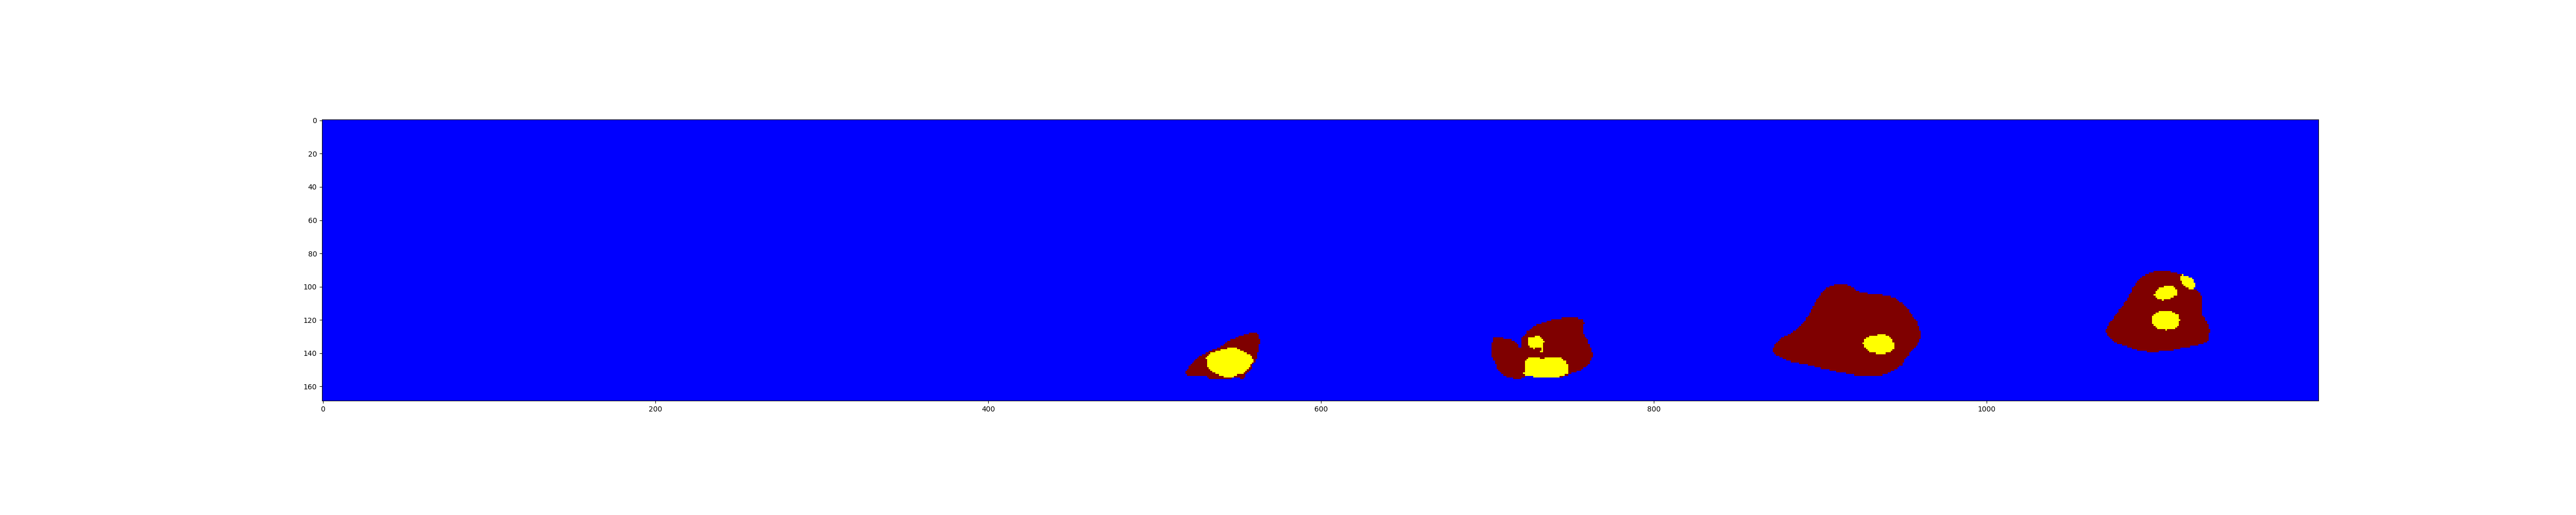
\includegraphics[width=\textwidth]{good_predicted.png}
		 	\caption{Good result} Top to bottom: input, ground truth, prediction \\
		 	IOU values for this specific data case: $0.9973$, $0.8823$, $0.7857$

		 	\label{fig:good}
		\end{figure} 
		\begin{figure}[htbp]
		 	\centering
		 	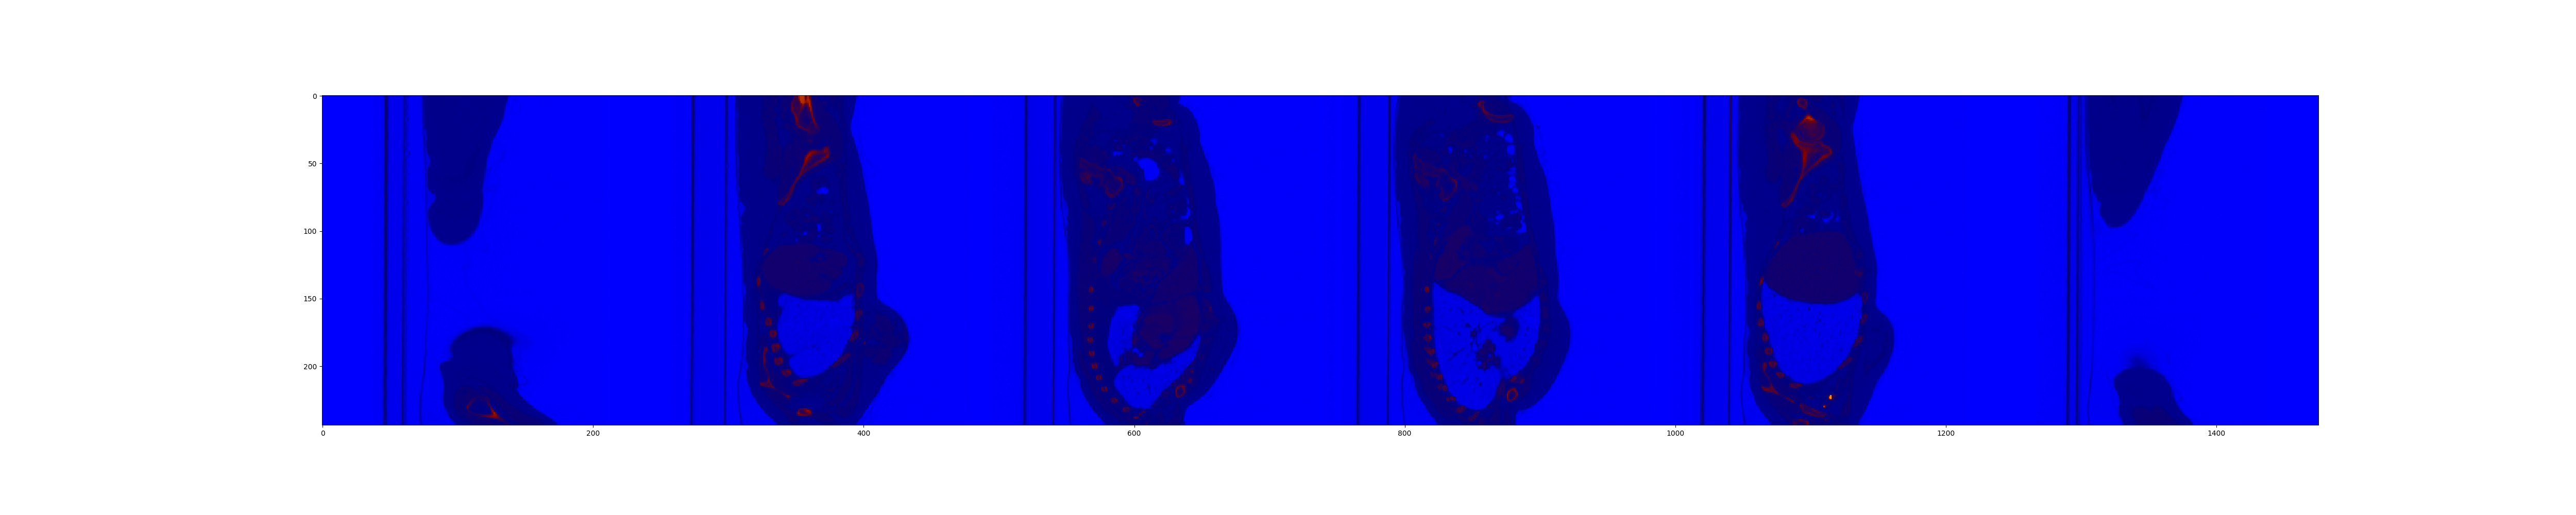
\includegraphics[width=\textwidth]{bad_input.png}\\
		 	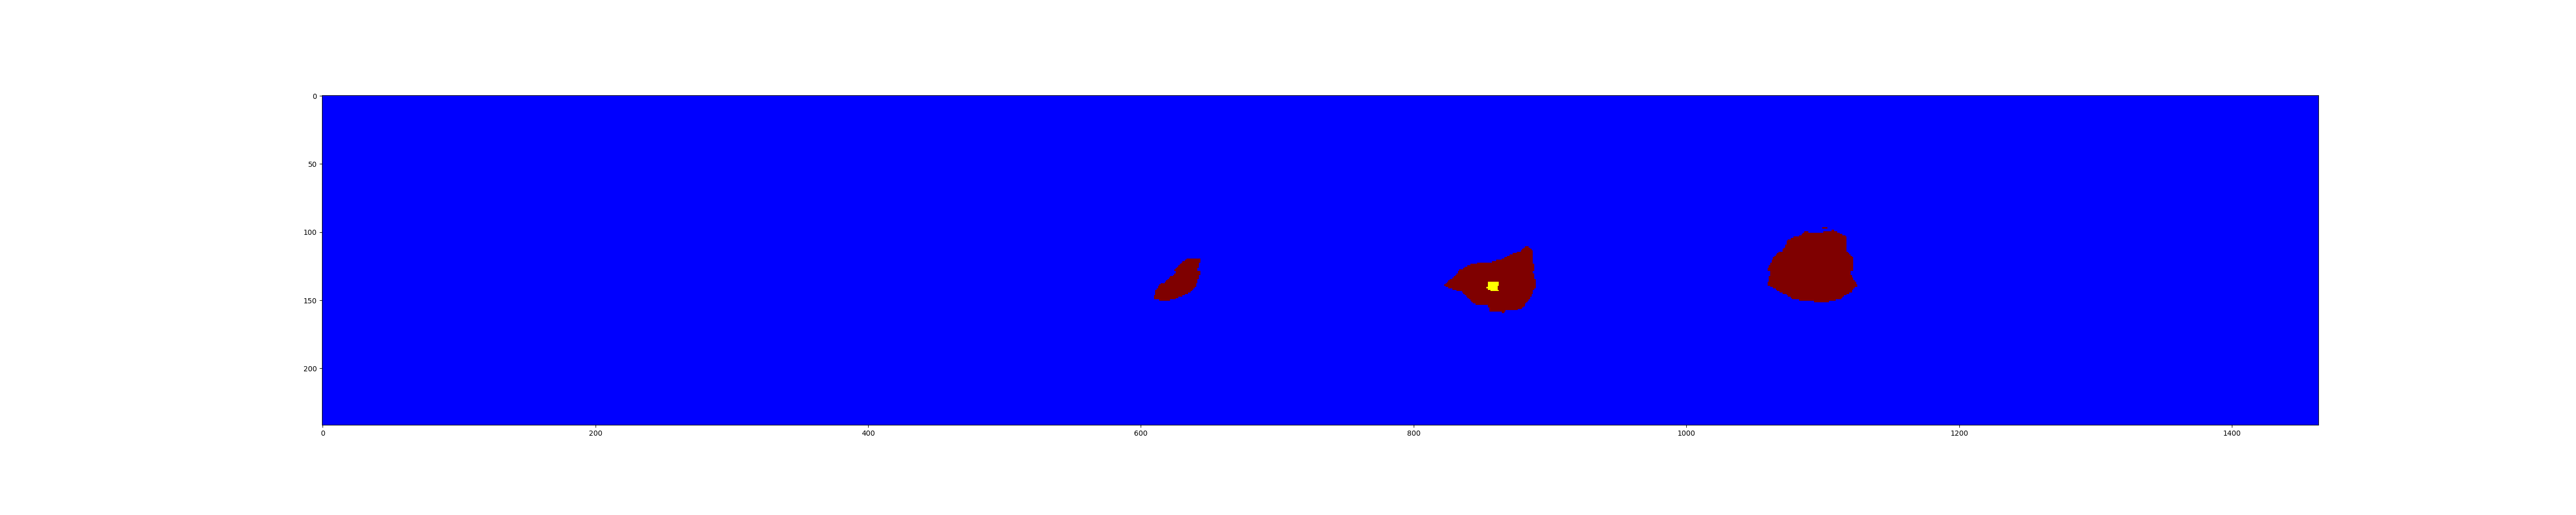
\includegraphics[width=\textwidth]{bad_target.png}\\
		 	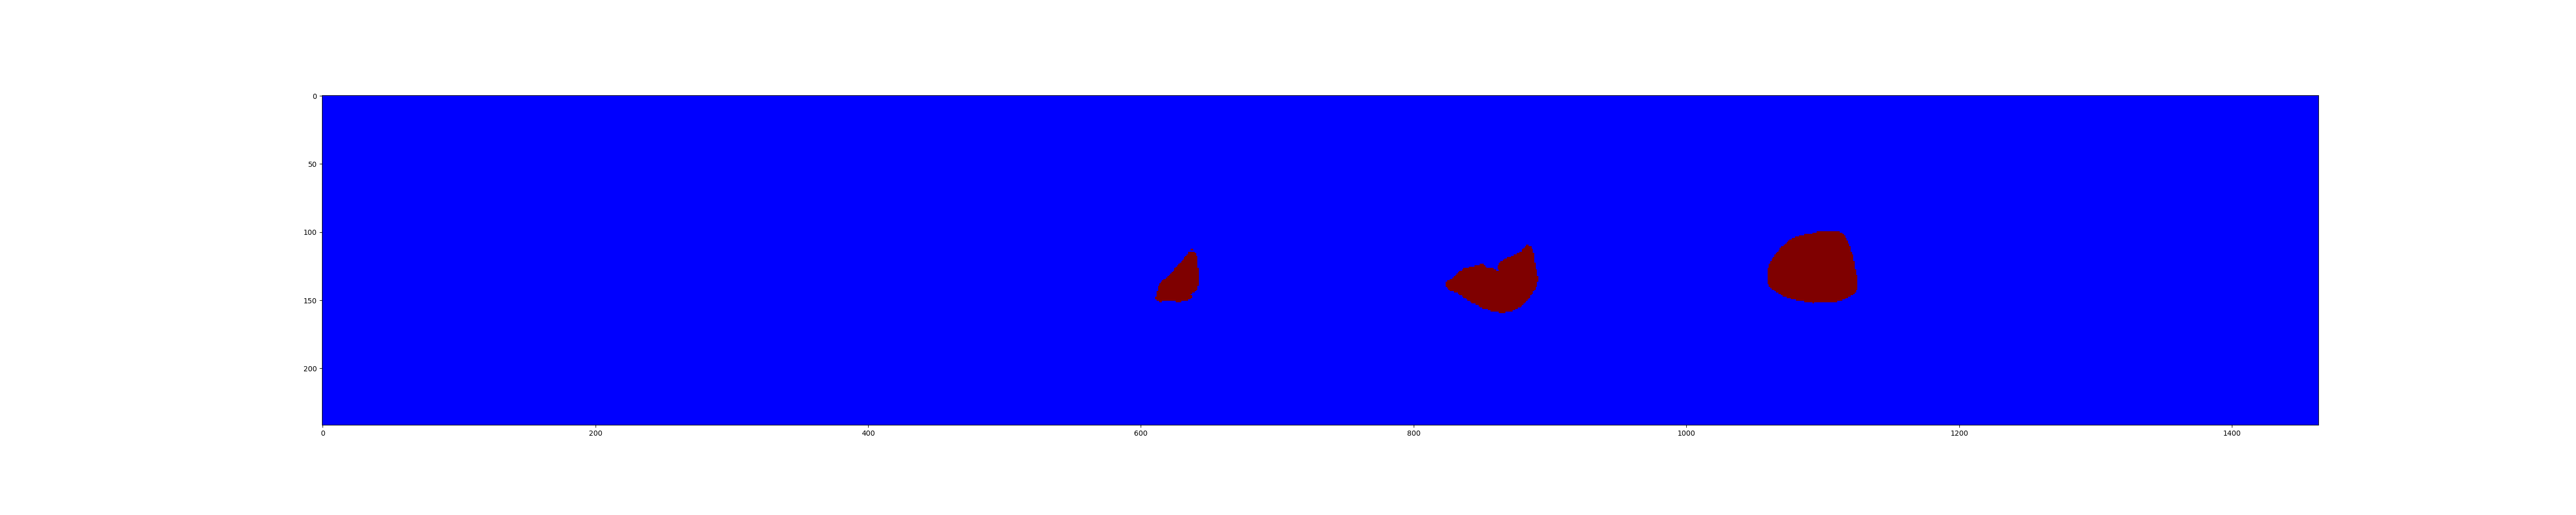
\includegraphics[width=\textwidth]{bad_predicted.png}
		 	\caption{Bad result} Top to bottom: input, ground truth, prediction \\
		 	IOU values for this specific data case: $0.9983$, $0.8666$, $0.3154$
		 	\label{fig:bad}
		\end{figure} 

		We also counted, how many voxels of which true class got (mis)classified as which other class. Here are the numbers for the two examples from figure~\ref{fig:good} and \ref{fig:bad}:

		For figure~\ref{fig:good}:

		\begin{tabular}{ | l | l || r | }
			\hline
			\textbf{True class} &
			\textbf{Predicted class} &
			\textbf{Number of voxels} \\ \hline
			0 (outside) & 0 (outside) & 6.534.266 \\ \hline
			0 (outside) & 1 (liver) & 5.467 \\ \hline
			0 (outside) & 2 (cancer) & 62 \\ \hline
			1 (liver) & 0 (outside) & 11.075 \\ \hline
			1 (liver) & 1 (liver) & 174.966 \\ \hline
			1 (liver) & 2 (cancer) & 4.650 \\ \hline
			2 (cancer) & 0 (outside) & 474 \\ \hline
			2 (cancer) & 1 (liver) & 2.146 \\ \hline
			2 (cancer) & 2 (cancer) & 26.894 \\ \hline
		\end{tabular}\\ \\

		For figure~\ref{fig:bad}:

		\begin{tabular}{ | l | l || r | }
			\hline
			\textbf{True class} &
			\textbf{Predicted class} &
			\textbf{Number of voxels} \\ \hline
			0 (outside) & 0 (outside) & 14.229.682 \\ \hline
			0 (outside) & 1 (liver) & 16.385 \\ \hline
			0 (outside) & 2 (cancer) & 0 \\ \hline
			1 (liver) & 0 (outside) & 6.853 \\ \hline
			1 (liver) & 1 (liver) & 154.104 \\ \hline
			1 (liver) & 2 (cancer) & 4 \\ \hline
			2 (cancer) & 0 (outside) & 0 \\ \hline
			2 (cancer) & 1 (liver) & 467 \\ \hline
			2 (cancer) & 2 (cancer) & 217 \\ \hline
		\end{tabular}

	\section{Problems and future tasks}

		We still need to do the same evaluation procedure for the prostate dataset, but we can reuse our existing code for that, so it should be done pretty quickly and easily.

\end{document}
